\documentclass[a4paper, 12pt, oneside]{scrbook}
\usepackage[style=authoryear,backend=biber]{biblatex}
%Farbige Tabelle
\usepackage[table,dvipsnames]{xcolor}
%\addbibresource{bibliography.bib}
\usepackage[ngerman]{babel}		
%=====Schrift============================
%\usepackage{helvet}
\usepackage{mathptmx} 
\renewcommand{\familydefault}{\rmdefault} 
%-----
\usepackage[T1]{fontenc}
\usepackage[utf8]{inputenc}
\usepackage{graphicx}
\usepackage{epstopdf}
\usepackage{float}
\usepackage{acronym}
\usepackage{booktabs}
\usepackage{caption}
\usepackage{csquotes}
\usepackage{fancyhdr}
\usepackage{url}
\usepackage{listings} 
\usepackage[datesep=.]{datetime2}
\DTMsetstyle{ddmmyy}
\usepackage[binary-units=true]{siunitx}
%Enforce pictures to be in the same section. Use \FloatBarrier before a new subsection to enforce it on subsection level.
\usepackage[section]{placeins}
%Landscape support for pdfs.
\usepackage{pdflscape}
\usepackage[subfigure]{tocloft}

%Settings for the header line
\newcommand{\defineHeader}{
\pagestyle{fancy}
\lhead{}
\chead{}
\rhead{\rightmark}
\renewcommand{\headrulewidth}{1pt}}


%Do not reset footnote numbering
\usepackage{chngcntr}
\counterwithout{footnote}{chapter}

\renewcommand{\lstlistoflistings}{\begingroup
\tocfile{\lstlistingname}{lol}
\endgroup}

%Selbst eingefügte
%TimesNewRoman
\usepackage{mathptmx}
\usepackage{lipsum,mathptmx,etoolbox}% http://ctan.org/pkg/{lipsum,mathptmx,etoolbox}
\makeatletter
\usepackage{subfigure} 

%Zeilenabstand auf 1,5 gesetzt
\usepackage[onehalfspacing]{setspace}
\usepackage{wrapfig}
\usepackage{tocbibind}
\usepackage{pdfpages}
\usepackage{enumitem}
\definecolor{tecrmigreen}{HTML}{1EA12D}
\definecolor{tecallianceBlue}{HTML}{193366}
%Zum durchgehenden Numerieren der Abbildungen
\usepackage{chngcntr}
\counterwithout{figure}{chapter}
\counterwithout{table}{chapter}
%Um SubSubSection auch numeriert zu bekommen
%\setcounter{secnumdepth}{3}

\usepackage{multirow}
\usepackage[right]{eurosym} 
\usepackage{longtable}

\usepackage{blindtext}
%Load hyperref at the end, otherwise it could be that the footnotes are broken
\usepackage[hidelinks]{hyperref}

\renewcommand*{\headfont}{\normalfont}
\renewcommand*{\multicitedelim}{\addsemicolon\space}
\renewcommand*{\headrulewidth}{0pt}
\renewcommand*{\arraystretch}{1.5}

\setlength{\parskip}{1.5ex}
% Absätze am Seitenende müssen mindestens drei Zeilen haben
\clubpenalties=3 10000 7500 2500
\widowpenalties=3 10000 7500 2500


%Listing
\usepackage{color}
\definecolor{gray}{rgb}{0.4,0.4,0.4}
\definecolor{darkblue}{rgb}{0.0,0.0,0.6}
\definecolor{cyan}{rgb}{.0,0.6,0.6}

%Farben Layout
\definecolor{backgroundWhite}{rgb}{1,1,1}
\definecolor{classesCyan}{rgb}{0.05, 0.545, 0.545}
\definecolor{keywordBlue}{rgb}{0.13,0.13,1}
\definecolor{commentGreen}{rgb}{0,0.5,0}
\definecolor{stringRed}{rgb}{0.7,0.05,0.05}
\definecolor{red}{rgb}{255,0,0}
\definecolor{borderGray}{rgb}{0.87,0.88,0.89}
\definecolor{brandBlue}{rgb}{0.30,0.50,0.74}
\definecolor{attributePurple}{rgb}{0.5,0.0,1}

%Farben für logische Einheiten
\definecolor{logicalUnitsBlue}{RGB}{85, 85, 255}
%\definecolor{logicalUnitsGreen}{RGB}{90, 255, 90}
\definecolor{logicalUnitsGreen}{RGB}{60, 190, 60}
\definecolor{logicalUnitsOrange}{RGB}{255, 165, 0}
\definecolor{logicalUnitsPink}{RGB}{255, 192, 203}

\lstset{
	basicstyle=\ttfamily,
	columns=fullflexible,
	showstringspaces=false,
	commentstyle=\color{gray}\upshape,
	numbers=left,
	%Um eine durchgehende Numerierung bei Listings zu erhalten
	numberbychapter=false
}



%Für das Anhangsverzeichnis
\makeatletter
\newcommand*{\maintoc}{% Hauptinhaltsverzeichnis
  \begingroup
    \@fileswfalse% kein neues Verzeichnis öffnen
    \renewcommand*{\appendixattoc}{% Trennanweisung im Inhaltsverzeichnis
      \value{tocdepth}=-10000 % lokal tocdepth auf sehr kleinen Wert setzen
    }%
    \tableofcontents% Verzeichnis ausgeben
  \endgroup
}
\newcommand*{\appendixtoc}{% Anhangsinhaltsverzeichnis
  \begingroup
    \edef\@alltocdepth{\the\value{tocdepth}}% tocdepth merken
    \setcounter{tocdepth}{-10000}% Keine Verzeichniseinträge
    \renewcommand*{\contentsname}{% Verzeichnisname ändern
      Anhang}%
    \renewcommand*{\appendixattoc}{% Trennanweisung im Inhaltsverzeichnis
      \setcounter{tocdepth}{\@alltocdepth}% tocdepth wiederherstellen
    }%
    \tableofcontents% Verzeichnis ausgeben
    \setcounter{tocdepth}{\@alltocdepth}% tocdepth wiederherstellen
  \endgroup
}
\newcommand*{\appendixattoc}{% Trennanweisung im Inhaltsverzeichnis
}
\g@addto@macro\appendix{% \appendix erweitern
  \if@openright\cleardoublepage\else\clearpage\fi% Neue Seite
  \phantomsection
  \addcontentsline{toc}{chapter}{\appendixname}% Eintrag ins Hauptverzeichnis
  \addtocontents{toc}{\protect\appendixattoc}% Trennanweisung in die toc-Datei
}

\g@addto@macro\appendix{%
  %\pagenumbering{Roman}%
  \addtocontents{toc}{\protect\renewcommand*{\protect\@pnumwidth}{3.5em}}%Seitenzahlen im Anhangverzeichnis nicht über Seitenrand hinaus. Problem entstand durch die langen römischen Zahlen. Siehe auch: http://www.komascript.de/node/608
}

\makeatother
\usepackage[toc,automake]{glossaries}
% Formatiere Glossareinträge:
\renewcommand{\glstextformat}[1]{\textbf{\em #1}}
%\renewcommand{\glstextformat}[1]{\textbf{\color{blue}\em #1}}

\usepackage{longtable}
\definecolor{tecrmigreen}{HTML}{1EA12D}
\definecolor{tecallianceBlue}{HTML}{193366}


%Custom Settings
%C# SourceCode format settings for listings
%\setmonofont{Consolas} %to be used with XeLaTeX or LuaLaTeX
\definecolor{bluekeywords}{rgb}{0,0,1}
\definecolor{greencomments}{rgb}{0,0.5,0}
\definecolor{redstrings}{rgb}{0.64,0.08,0.08}
\definecolor{xmlcomments}{rgb}{0.5,0.5,0.5}
\definecolor{types}{rgb}{0.17,0.57,0.68}



\setlength{\parindent}{0em} 

\addbibresource{bibliography.bib}

\makeglossaries
\makeindex
\begin{document}


\chapter{Funktion zur Berechnung der Kreuz-Korrelation}
Das Python Skript \enquote{func\_cross\_correlation.py} bietet als Einstiegspunkt die Funktion\\ \mbox{\enquote{crossCorrelation(...)}} an. Im Folgenden werden die Parameter und deren Bedeutung beschrieben.

\section{Beschreibung der Parameter}
Manche der Parameter sind optional, während andere angegeben werden müssen.
\subsection{Pflichtparameter}
Es gibt nur zwei Parameter, die beim Aufruf der Funktion mitgegeben werden müssen. Dabei handelt es sich um die beiden Sequenzen, die verarbeitet werden sollen.
\begin{description}[style=nextline]
\item[seqA] Die erste Datensequenz in Form eines eindimensionalen Arrays. Die enthaltenen Zahlenwerte müssen in Float konvertierbar sein.
\item[seqB] Die zweite Datensequenz in Form eines eindimensionalen Arrays. Die enthaltenen Zahlenwerte müssen in Float konvertierbar sein.
\end{description}

\subsection{Optionale Parameter}
Folgende Parameter sind optional:
\begin{description}[style=nextline]
\item[plotNormalizedData] [Default: False] Auf True setzen, wenn die beiden Sequenzen auch normalisiert dargestellt werden sollen.
\item[plotCorrelations] [Default: False] Auf True setzen, wenn die berechnete Kreuz-Korrelation dargestellt werden soll. Dabei werden alle drei Berechnungsmethoden \enquote{Valid}, \enquote{Same} und \enquote{Full} dargestellt.
\item[plotNonNormalizedResults] [Default: False] Auf True setzen, wenn auch die unnormalisierten Ergebnisse dargestellt werden sollen.
\item[plotNormalizedResults] [Default: True] Auf False setzen, wenn auch die normalisierten Ergebnisse nicht dargestellt werden sollen.
\item[subtractMeanFromResult] [Default: True] Auf False setzen, wenn das arithmethische Mittel nicht von den Ergebnissen abgezogen werden soll.
\end{description}

\section{Beispiel Ergebnisse}
Es gilt für alle Beispiele (solange nicht im Beispiel spezifiziert):\\
Vorbedingung: Zwei Sequenzen mit je 10000 Einträgen. \\
SeqA:
\[ a_{n} =
  \begin{cases}
    1       & \quad \text{wenn } n \text{ enthalten in [1005,2005,1505,3505,5505,6005,6505,8005,8505,9005]}\\
    0  & \quad \text{sonst}
  \end{cases}
\]
SeqB:
\[ b_{n} =
  \begin{cases}
    1       & \quad \text{wenn } n \text{ enthalten in [1000,2000,1500,3500,5500,6000,6500,8000,8500,9000]}\\
    0  & \quad \text{sonst}
  \end{cases}
\]
Es ist ersichlich, dass die Sequenzen zueinander um einen Index von 5 verschoben sind.

\subsection{Nur Pflichtparameter angegeben}
Der Aufruf der Funktion ohne optionale Parameter, liefert für die Beispielsequenzen folgendes Ergebnis (dargestellt in Abbildung~\ref{fig:correlationDefaultParams}):
\begin{figure}[H]
    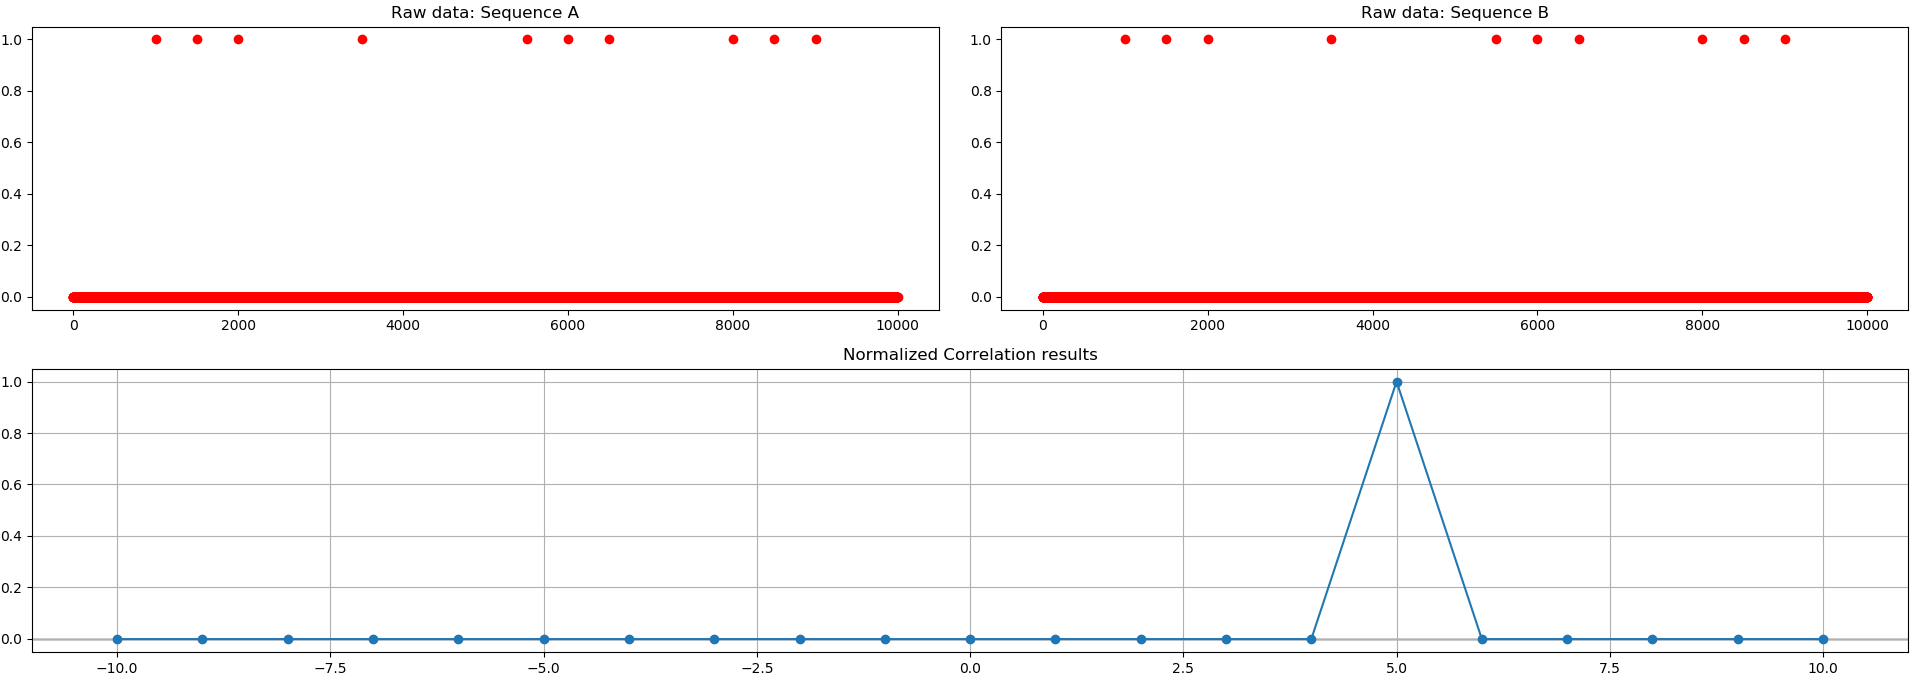
\includegraphics[width=\linewidth]{./images/correlationDefaultParams.PNG}
    \caption{Ergebnis der Funktion bei Default-Parametern.}
    \label{fig:correlationDefaultParams}
  \end{figure}


\subsection{Optionaler Parameter: plotNormalizedData}
Durch setzen des optionalen Parameters \enquote{plotNormalizedData} auf True, werden die beiden Sequenzen, zusätzlich in normalisierter Form dargestellt. 
Siehe dazu Abbildung~\ref{fig:correlationPlotNormalizedData}. 
\begin{figure}[H]
    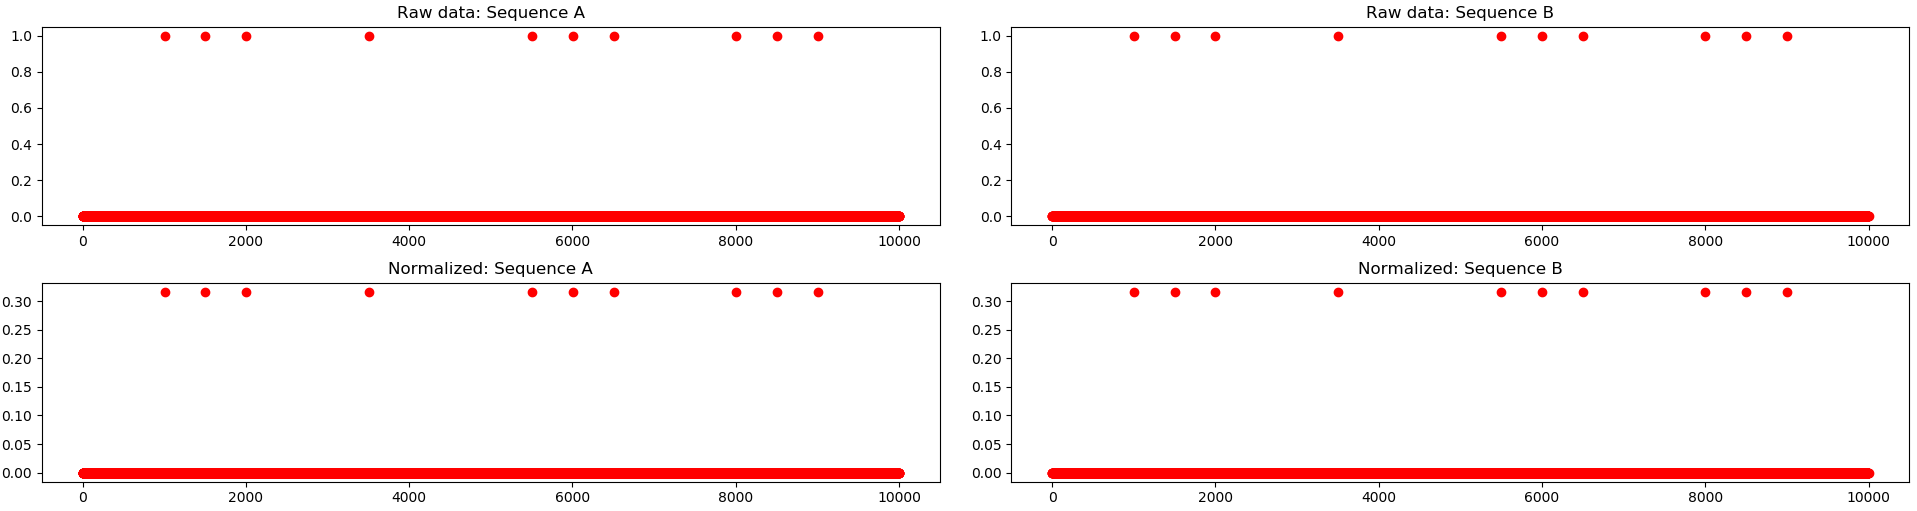
\includegraphics[width=\linewidth]{./images/correlationPlotNormalizedData.PNG}
    \caption{Ergebnis der Funktion bei \enquote{plotNormalizedData = True} (Darstellung der Ergebnisse weggelassen). }
    \label{fig:correlationPlotNormalizedData}
  \end{figure}

\subsection{Optionaler Parameter: plotCorrelations}
Durch setzen des optionalen Parameters \enquote{plotCorrelations} auf True, 
wird die Kreuz-Korrelation der beiden Sequenzen berechnet.
Dabei werden alle drei Berechnungsmethoden \enquote{Valid}, \enquote{Same} und \enquote{Full} dargestellt.
Siehe dazu Abbildung~\ref{fig:correlationPlotCorrelations}. 
\begin{figure}[H]
    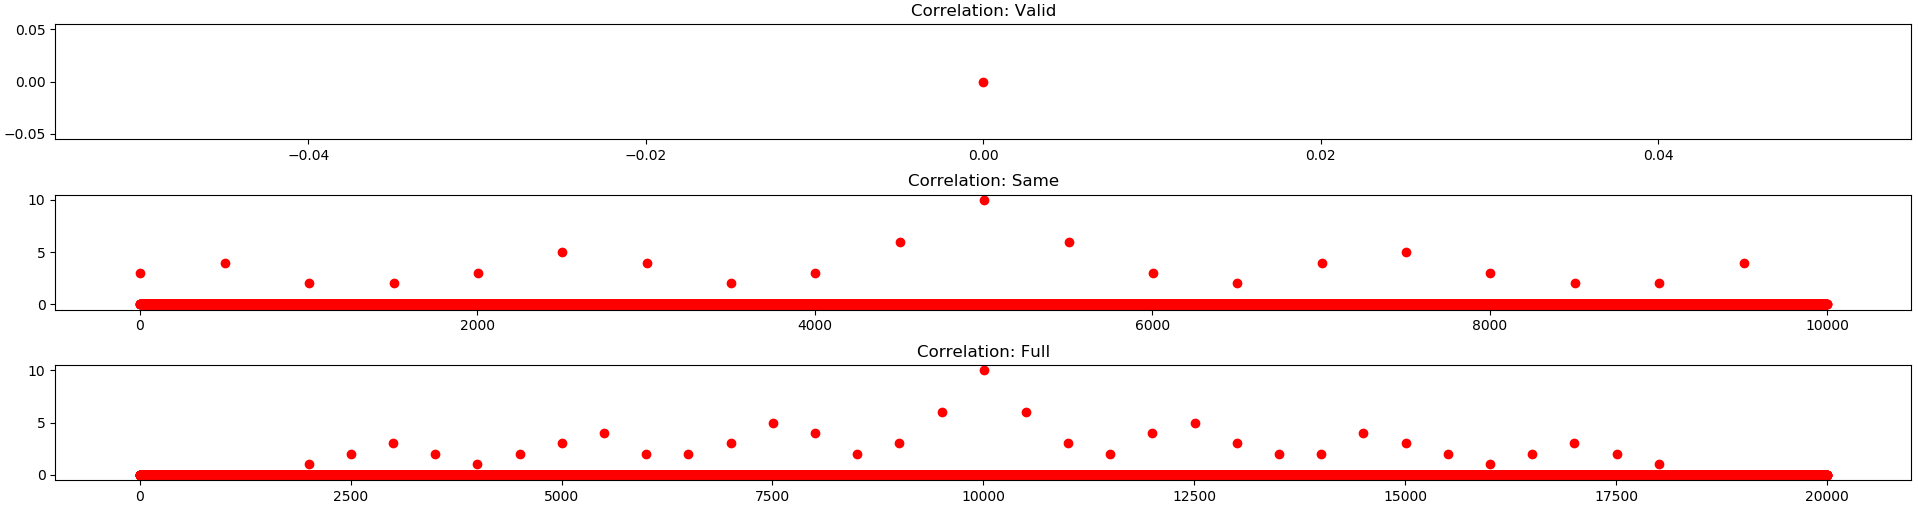
\includegraphics[width=\linewidth]{./images/correlationPlotCorrelations.PNG}
    \caption{Zusätzliche Ausgabe der Funktion bei \enquote{plotCorrelations = True} (Darstellung der Ergebnisse weggelassen). }
    \label{fig:correlationPlotCorrelations}
  \end{figure}

\subsection{Optionaler Parameter: plotNonNormalizedResults}
Durch setzen des optionalen Parameters \enquote{plotNonNormalizedResults} auf True, können die Ergebnisse zusätzlich in unnormalisierter Form ausgegeben werden.
Siehe dazu Abbildung~\ref{fig:correlationPlotNonNormalizedResults}. 
\begin{figure}[H]
    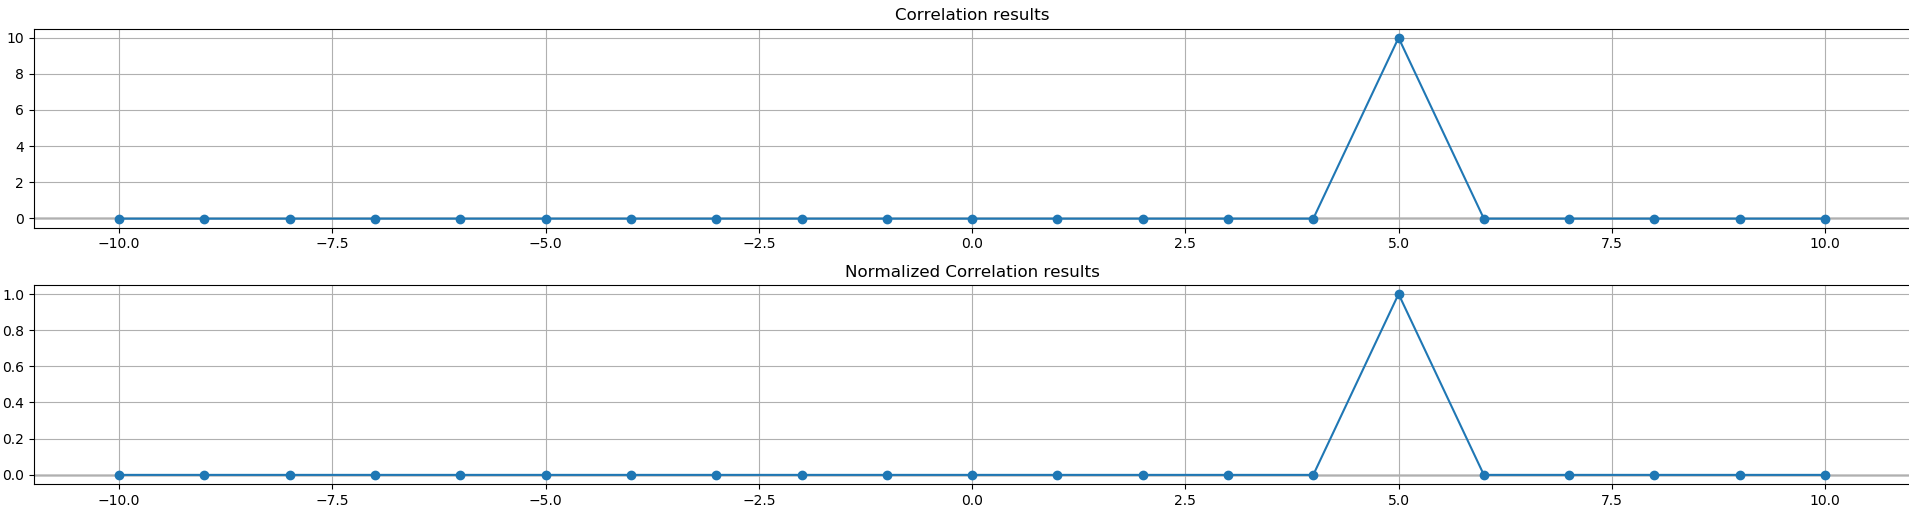
\includegraphics[width=\linewidth]{./images/correlationPlotNonNormalizedResults.PNG}
    \caption{Zusätzliche Ausgabe der Funktion bei \enquote{plotNonNormalizedResults = True}. }
    \label{fig:correlationPlotNonNormalizedResults}
  \end{figure}

\subsection{Optionaler Parameter: plotNormalizedResults}
Durch setzen des optionalen Parameters \enquote{plotNormalizedResults} auf False, kann die Ausgabe der normalisierten Ergebnisse verhindert werden.

\subsection{Optionaler Parameter: subtractMeanFromResult}
Um die Auswirkung des Parameters darzustellen, werden folgende Sequenzen vorrausgesetzt (je 10000 Einträge):\\
SeqA:
\[ a_{n} =
  \begin{cases}
    2       & \quad \text{wenn } n \text{ enthalten in [1005,2005,1505,3505,5505,6005,6505,8005,8505,9005]}\\
    1  & \quad \text{sonst}
  \end{cases}
\]
SeqB:
\[ b_{n} =
  \begin{cases}
    2       & \quad \text{wenn } n \text{ enthalten in [1000,2000,1500,3500,5500,6000,6500,8000,8500,9000]}\\
    1  & \quad \text{sonst}
  \end{cases}
\]
Die Sequenzen sind wieder um einen Wert von 5 verschoben, allerdings wechseln diese nicht zwischen 0 und 1, sondern zwischen 1 und 2. 
Die Ergebnisse können dabei unübersichtlich werden, deshalb wird ohne Angabe des Parameters, True als Standardwert verwendet.
Dadurch wird das arithmethische Mittel des Ergebnis vom Ergebnis selbst abgezogen. Abbildung~\ref{fig:correlationSubtractMeamFromResultTrue} 
und \ref{fig:correlationSubtractMeamFromResultFalse} zeigen die Auswirkung des Parameters. 
\begin{figure}[H]
    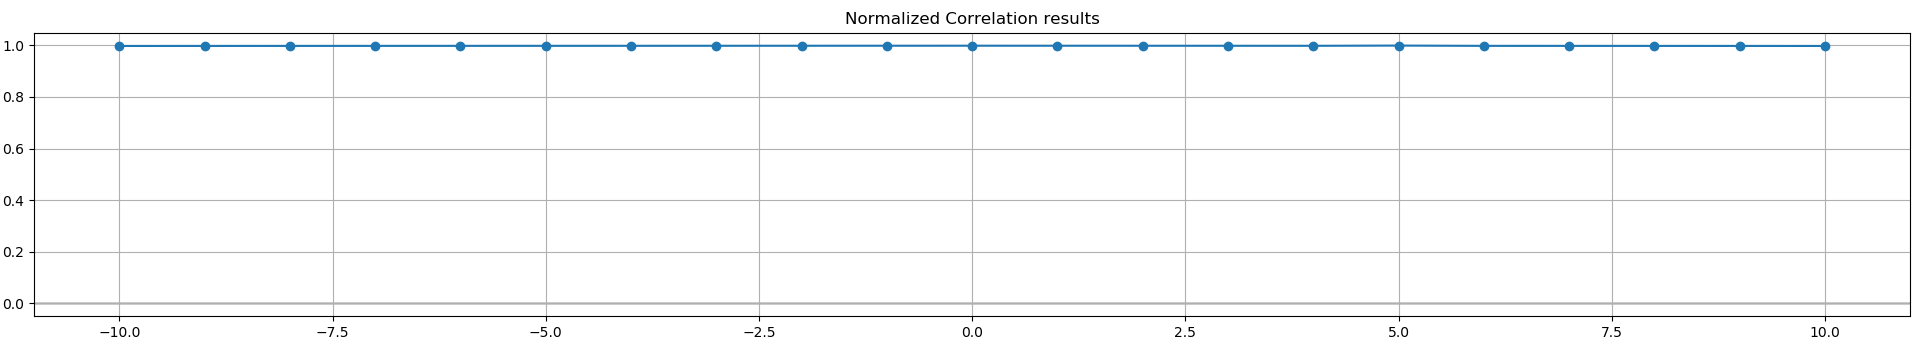
\includegraphics[width=\linewidth]{./images/correlationSubtractMeamFromResultFalse.PNG}
    \caption{Darstellung des Ergebnis bei \enquote{subtractMeanFromResult = False}. Ausschläge sind sehr schwer erkennbar. }
    \label{fig:correlationSubtractMeamFromResultFalse}
  \end{figure}

  \begin{figure}[H]
    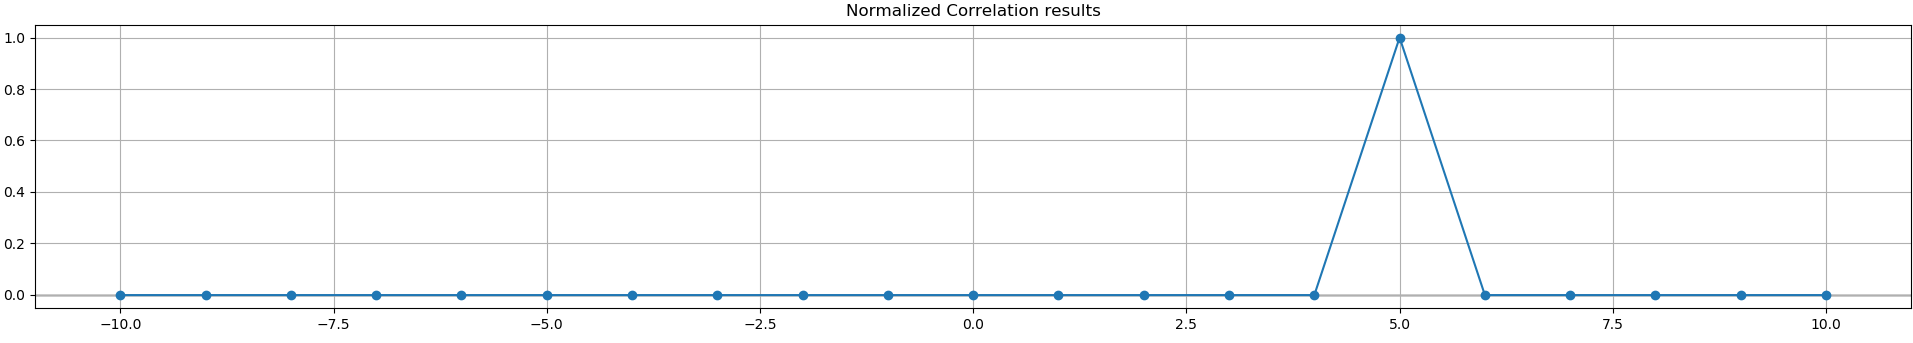
\includegraphics[width=\linewidth]{./images/correlationSubtractMeamFromResultTrue.PNG}
    \caption{Darstellung des Ergebnis bei \enquote{subtractMeanFromResult = True}. Ausschläge sind besser erkennbar. }
    \label{fig:correlationSubtractMeamFromResultTrue}
  \end{figure}


\chapter{Suche nach Pattern mit Hilfe der Kreuz-Korrelation}
Das Python Skript \enquote{func\_cross\_correlation\_patternsearch.py} bietet zwei Funktionen an, die verwendet werden können, 
um nach einem gegebenen Pattern in einer Sequenz zu suchen.

\section{Angebotene Funktionen}
Folgende Funktionen werden angeboten:

\subsection{Funktion: getCorrelationDataForPatternSearch}
Mit Hilfe der \enquote{getCorrelationDataForPatternSearch} Funktion kann nach einem Pattern in einer gegebenen Sequenz gesucht werden. Dafür sind folgende Parameter nutzbar:
\begin{description}
    \item[seqA] Die Sequenz in der nach dem Pattern gesucht werden soll. Übergeben in Form eines eindimensionalen Arrays. Die enthaltenen Zahlenwerte müssen in Float konvertierbar sein.
    \item[pattern] Das Pattern nach dem gesucht werden soll. Übergeben in Form eines eindimensionalen Arrays. Die enthaltenen Zahlenwerte müssen in Float konvertierbar sein.
    \item[plotCorrelation] [Default: False] Auf True setzen, wenn die berechnete Kreuz-Korrelation dargestellt werden soll.
\end{description}
Die Funktion gibt die berechnete Kreuz-Korrelation zurück, die in der nächsten Funktion \enquote{extractIndicesFromCorrelationData} verwendet werden kann.

\subsection{Funktion: extractIndicesFromCorrelationData}
Die Funktion kann verwendet werden, um die Indizes zu berechnen, an denen das Pattern in der Sequenz auftritt. Dafür muss der Funktion das Ergebnis der \enquote{getCorrelationDataForPatternSearch} Funktion
übergeben werden. Als Rückgabe erhält man die Indizes und der Wert der Korrelation an dieser Stelle.\\
Optional kann ein Schwellwert übergeben werden. Je nachdem wie dieser Schwellwert gewählt ist, werden mehr oder weniger Indizes zurückgegeben. Bei einem hohen Schwellwert wird 
jeweils nur der erste Index zurückgegeben, bei dem das Pattern auftritt. Bei einem niedriger gewählten Schwellwert werden alle Indizes zurückgegeben, an denen das Pattern auftritt. 

\subsection{Beispiel für die Pattern-Suche}
Vorbedingung: Eine Sequenzen mit 10000 Einträgen. \\
SeqA:
\[ a_{n} =
  \begin{cases}
    1       & \quad \text{wenn } n \text{ enthalten in [1005,1007,1010,6005,6007,6010]}\\
    0  & \quad \text{sonst}
  \end{cases}
\]
Gesuchtes Pattern:
\[
pattern = [1,0,1,0,0,1,0] 
\]
Das Pattern tritt in der gegeben Sequenz zwei Mal auf (an Index 1005 und 6005).
Der Aufruf der \enquote{getCorrelationDataForPatternSearch} Funktion mit dem \enquote{plotCorellation = True} zeigt die in Abbildung~\ref{fig:patternsearchCorrelation} dargestellte Kreuz-Korrelation.

\begin{figure}[H]
  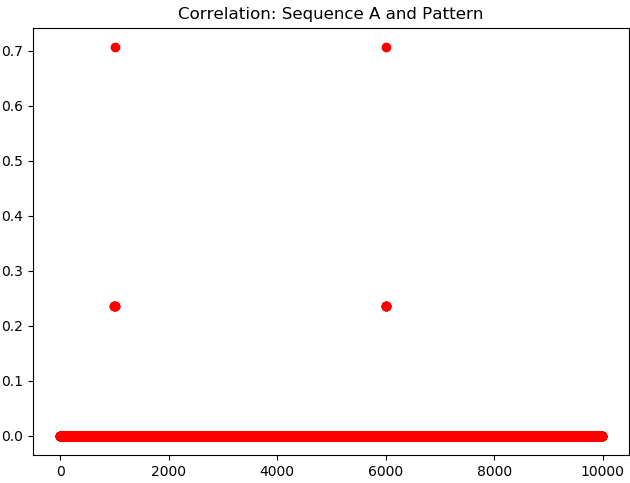
\includegraphics[width=\linewidth]{./images/patternsearchCorrelation.PNG}
  \caption{Kreuz-Korrelation der Patternsuche.}
  \label{fig:patternsearchCorrelation}
\end{figure}

\begin{samepage}
Mit Hilfe der dargestellten Kreuz-Korrelation kann der Schwellwert für die \enquote{extractIndicesFromCorrelationData} festgelegt werden.
Ein Aufruf mit einem Schwellwert von \enquote{0.3} liefert folgendes Ergebnis: \\
\begin{align*}
   & [6005, 0.70710678], \\
   & [1005, 0.70710678]
\end{align*}

Dabei handelt es sich um die Indizes, an denen das Pattern in der Sequenz beginnt (inklusive den Wert an dieser Stelle). \\
\end{samepage}
\begin{samepage}
Ein Aufruf mit einem Schwellwert von \enquote{0.2} liefert dagegen folgendes Ergebnis: \\
\begin{align*}
  &  [6005, 0.70710678], \\
  & [1005, 0.70710678], \\
  & [6003, 0.23570226], \\
  & [1000, 0.23570226], \\
  & [6007, 0.23570226], \\
  & [6010, 0.23570226], \\
  & [6002, 0.23570226], \\
  & [6000, 0.23570226], \\
  & [1010, 0.23570226], \\
  & [1008, 0.23570226], \\
  & [1007, 0.23570226], \\
  & [1003, 0.23570226], \\
  & [1002, 0.23570226], \\
 & [6008, 0.23570226]
\end{align*}
Darin enthalten sind Indizes im Bereich von 1000 bis 1010 sowie 6000 bis 6010. Die Bereiche sind größer als das Pattern selbst, allerdings ist das Pattern in diesen Bereichen enthalten.
\end{samepage}

\end{document}
